\cotefile{157-4}
\scanpage{363}
\mspage{87}
\unsure{distincts|distincte} de $\mathbb W_\infty$. Je n'ai pas même prouvé que $W_{\unsure{\omega|w}}\ne\mathbb W_\infty$, alors que je n'ai pas le moindre doute que tel est bien le cas. A fortiori, j'ignore si le plus petit localiseur fond. satisfaisant $\mathrm{Loc}(7\mathrm{D}_{W_\omega})$\deleted{\unsure{,}} est $\ne\mathbb W_\infty$. Je serais tout particulièrement intéressé par le plus petit localiseur $\widetilde{\mathbb W}_\infty\subset\mathbb W_\infty$ satisfaisant tous les axiomes de stabilité $\mathrm{Loc}(1\,\mathrm{ter},2,3\,\mathrm{bis},4,6\deleted{\unsure{\mathrm{bis}}},7,8)$ (\uline{NB} il satisfait nécessairement $\mathrm{Loc}(5)$ car $\widetilde{\mathbb W}_\infty\subset\mathbb W_\infty\subset\mathbb W_0$\deleted{\unsure{)}}, de plus $\mathrm{Loc}(7)$ équivaut, en présence de $\mathrm{Loc}(8)$, à la forme très faible $\mathrm{Loc}(7\mathrm{D}_{W_\omega})$ : $\unsure{\mathrm{Parf}}_{W_\omega}\cap W\subset W^{\unsure{\mathrm{ni}|\mathrm{ui}}}$. Enfin, on montre que $4$ est conséquence des autres axiomes, cf plus bas.)

Je conjecture à présent que $\widetilde{\mathbb W}_\infty$ (qui donne lieu à un formalisme homotopique \deleted{\unsure{tout}} aussi complet que \deleted{$\mathbb W_\infty$} les \unsure{sempiternelles|sempiternelle} ``équivalences faibles'') est bel et bien $\ne\mathbb W_\infty$. Et je suspecte
% archive sheet number: 362
\scanpage{364}
\mspage{88}
que la catégorie $\mathrm{Hot}_{\widetilde{\mathbb W}_\infty}$ mérite d'être appelée catégorie des ``\uline{types d'homotopie simples}'' (à la Whitehead)\textsuperscript{*}.%
% slanted
\margin{\unsure{Canulé|Annulé} (\unsure{?!}), cf commentaire 6.5 page 92.} Un premier test décisif, c'est de vérifier que l'invariant ``\unsure{chronologique|cohomologique} principal de Whitehead d'un type d'\deleted{\unsure{R}}hom. simple, à savoir un élément dans un $K(\mathbb Z(\pi_1))$ (si je me rappelle bien)\textsuperscript{*} -- ou quelque
% slanted
\margin{non, c'est un invariant plus fin\ldots} chose d'approchant, peut se définir déjà en termes \inserted{des objets} de $\mathrm{Hot}_{\bullet\widetilde{\mathbb W}_\infty}$ (le $\mathrm{Hot}$ pointé)\textsuperscript{*}. Et d'abord, si on associe à une \deleted{\unsure{espace} \inserted{\unsure{avec}} \unsure{triang.}} ``maquette simpliciale'' finie (\unsure{décrivant|divisant} \unsure{combinatoirement} une triangulation \unsure{finie}) l'ens. ordonné de ses simplexes, vu comme un objet de $\mathrm{Cat}$, l'objet correspondant de $\mathrm{Hot}_{\widetilde{\mathbb W}_\infty}$, celui-ci ne change pas\textsuperscript{*}, à
% slanted
\margin{C'est évident \unsure{$=$|même} pour $W_{\unsure{\omega|w}}$, puisque le type d'homotopie \uuline{\unsure{strict|stricte}} \uline{ne change} pas ! Non, \unsure{il y a|s'il y a} \unsure{ici} confusion entre homotopie \unsure{topologique} et homotopie \unsure{combinatoire|combinatoires}, p. 92\ldots} isom. can. près, quand on \deleted{\unsure{remplace}} \inserted{effectue} sur \deleted{\unsure{la}} le ``polyèdre'' envisagé une opération élé%
% archive sheet number: 363
\scanpage{365}%
\mspage{89}%
mentaire à la Whitehead. Cela suggère d'ailleurs d'essayer de définir de telles opérations élémentaires dans $\mathrm{Cat}$ \deleted{tout} \unsure{entier}, ou \inserted{tout au moins} dans la \deleted{\unsure{cat.}} sous-catégorie des \inserted{(petits)} ensembles ordonnés, \deleted{\unsure{pour|par}} dans l'espoir de parvenir (peut-être) à une construction plus directe du localiseur pertinent pour le type d'homotopie simple.

c) Je termine par un commentaire sur le sens de l'axiome $\mathrm{Loc}(7\mathrm{D}_{W_{\unsure{\omega|w}}})$, par opposition avec l'axiome plus \unsure{faible} $\mathrm{Loc}(7\mathrm{F})$ qui assure seulement l'existence d'une ``structure à fibrations'' : $(W,\mathrm{Fib}_W)$ sur $\mathrm{Cat}$ -- Je signale \deleted{\unsure{aussi}} en passant que $\mathrm{Loc}(7\mathrm{F})$ tout comme $\mathrm{Loc}(5)$ et comme $\mathrm{Loc}(9)$, et à la différence de tous les autres axiomes passés en revue jusqu'à présent, n'est \uline{pas} un axiome de stabilité : il affirme, non que certaines flèches (sous des hypo convenables) sont dans $W$, mais l'existence d'une factorisation. Aussi il n'est
% archive sheet number: 364
\scanpage{366}
\mspage{90}
nullement clair que l'intersection de deux localiseurs fond. satisfaisant à $\mathrm{Loc}(7\mathrm{F})$ y satisfasse.

$\mathrm{Loc}(7\mathrm{D}_{W_{\unsure{\omega|w}}})$ est exactement ce qu'il faut pour assurer que la factorisation canonique d'une flèche $f:X\unsure{-|\to}Y$ de $\mathrm{Cat}$ en $f=pi$, avec $i\in W_\omega$, $p\in\mathrm{Parf}_{W_\omega}$, est aussi une factorisation \deleted{\unsure{de}} \unsure{du} type stipulé par l'axiome de factorisation $\mathrm{Loc}(7\mathrm{F})$ : \unsure{on a|car.} (bien sûr) $i\in W$, mais aussi $p\in\mathrm{Fib}_W$ (car $\mathrm{D}_{W_\omega}$ équivaut à sa forme forte $\mathrm{Parf}_{W_\omega}\subset\mathrm{Fib}_W$). Cela signifie aussi que la factorisation canonique de $f$ peut être utilisée pour ``calculer'' ses fibres homotopiques, non seulement en les points de $Y$, mais aussi \unsure{p.r.} à un morphisme de chgt. de base $Y'\unsure{\longrightarrow|\Longrightarrow}Y$. \deleted{\unsure{?}}

En l'absence de cet axiome,
% archive sheet number: 365
\scanpage{367}
\mspage{91}
admettant seulement $\mathrm{Loc}(7\mathrm{F})$, on sait qu'il existe une théorie des fibres $W$-homotopiques, mais on n'a \inserted{a priori} aucun moyen pratique pour ``calculer'' les\inserted{dites} fibres, faute de disposer d'un critère maniable \inserted{suffisant} pour assurer $p\in\mathrm{Fib}_W$. \deleted{\unsure{Je}}J'ai donc l'impression que l'axiome $\mathrm{Loc}(7\mathrm{F})$ ne va être d'un maigre usage. (Il est vrai que l'exemple de $\mathbb W_0$ devrait me rendre prudent ! Il me faudrait regarder le cas des $\mathbb W_{\unsure{n|m}}$, s'ils satisfont $\mathrm{Loc}(7\mathrm{F})$\ldots.)

À mon sens, l'axiome $\mathrm{Loc}(7\mathrm{D}_{W_{\unsure{\infty|\omega|w}}})$ est le \inserted{l'exact} ``minimum vital'' pour \deleted{\unsure{avoir}} être à l'aise dans le maniement des fibres $W$-homotopiques. Il est remarquable que ceci implique qu'on doive avoir $W\subset\mathbb W_\infty$, et que cela exclut du même coup \deleted{\uline{toutes}} les variantes considérées à ce jour de la notion du type d'homotopie !
% archive sheet number: 366
\scanpage{368}
\mspage{92}
\unsure{6.5.|P.S.} Finalement, la relation entrevue avec les ``types d'homotopie simples'' de Whitehead s'évanouit\textsuperscript{*} : en effet, ces derniers sont strictement
% slanted
\margin{Mais peut-être quand même, -- la question reste ouverte.} plus fins que les types d'homotopie (\uline{stricts}) ordinaires, et l'invariant de Whitehead n'est \uline{pas} un invariant du type d'homotopie ordinaire. Il est vrai que lorsqu'on considère le squelette simplicial d'un polyèdre triangulé comme objet de $\mathrm{Cat}$, l'homotopie (continue) ordinaire entre deux tels polyèdres s'interprète, dans $\mathrm{Cat}$, non pas \deleted{\unsure{(contr.}} (me semble-t-il) par l'existence d'un homotopisme\deleted{\unsure{,}} entre les objets correspondants de $\mathrm{Cat}$, mais par leur isomorphie dans $\mathrm{Hot}_{\mathbb W_\infty}\overset{\mathrm{def}}{=}\mathrm{Cat}(\mathbb W_\infty)^{-1}$. Mais le procédé d'approximations simpliciales de Brouwer montre que si les polyèdres $X$ et $Y$ sont homotopes, alors il existe des subdivisions simpliciales \inserted{$X',Y'$} de $X$ et de $Y$ qui sont ``combinatoirement homotopes'' (dans un sens convenable). Donc \deleted{question qui \unsure{s'apprête|s'impose}} je présume que les maquettes simpliciales de $X'$ et de $Y'$ sont alors homotopes dans $\mathrm{Cat}$. Il s'ensuivrait que
% archive sheet number: 367
\scanpage{369}
\mspage{93}
$X$ et $Y$, j'entends leurs maquettes, sont bien homotopes dans $\mathrm{Cat}$, s'il est vrai qu'une subdivision simpliciale (il suffirait : la subdivision barycentrique, \inserted{en itérant\ldots}) \deleted{\unsure{de}} de $X$ \deleted{\unsure{est}}\unsure{a} une maquette dans $\mathrm{Cat}$ qui lui est homotope. La question soulevée ici me paraît intéressante, il faut visiblement en trouver la réponse. Elle se pose déjà pour \deleted{tout} ensemble ordonné $I$, qu'on va supposer fini pour simplifier, en prenant l'ensemble (ordonné \inserted{par inclusion}) $I'=\mathrm{sd}(I)$ des parties totalement ordonnées de $I$. On sait que les réalisations topologiques de $I$ et de $\mathrm{sd}(I)$ sont canoniquement \unsure{homéomorphes}, mais $I$ et $\mathrm{sd}(I)$ sont-ils homotopes dans $\mathrm{Cat}$ ? On a bien une application croissante

\[
 \text{can.}\qquad f:\mathrm{sd}(I)\longrightarrow I,
\]

qui associe à toute partie tot. ordonnée de $I$ son plus grand élément. Mais existe-t-il une \unsure{application} croissante en sens inverse, qui soit un homotopisme inverse du précédent à homotopie près ?

\deleted{\unsure{Je}} Je viens de vérifier dans le cas
% archive sheet number: 368
\scanpage{371}
\mspage{95}
du bord du $2$-simplexe

\figure{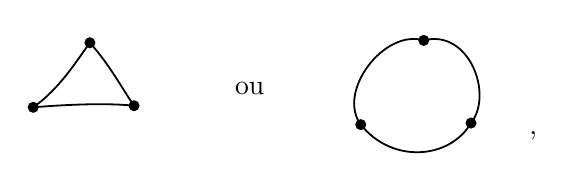
\begin{tikzpicture}[x=1cm,y=1cm,line width=.65pt]
\draw (0,0) .. controls (.34,.24) and (.55,.59) .. (.72,.82) .. controls (.97,.54) and (1.11,.27) .. (1.28,.02) .. controls (.91,.06) and (.36,.03) .. cycle;
\fill (0,0) circle (2pt) (.72,.82) circle (2pt) (1.28,.02) circle (2pt);
\node at (2.75,.24) {ou};
\draw (4.16,-.22) .. controls (3.85,.20) and (4.46,1.00) .. (4.96,.85) .. controls (5.53,1.00) and (5.85,.17) .. (5.56,-.20) .. controls (5.29,-.66) and (4.56,-.72) .. cycle;
\fill (4.16,-.22) circle (2pt) (4.96,.85) circle (2pt) (5.56,-.20) circle (2pt);
\node at (6.35,-.36) {,};
\end{tikzpicture}}

subdivision barycentrique

\figure{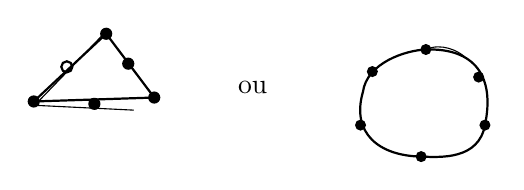
\begin{tikzpicture}[x=1cm,y=1cm,line width=.8pt]
\draw (0,0) -- (.92,.86) -- (1.53,.05) -- cycle;
\draw[thin] (.02,-.04) -- (.88,.85) (.04,-.05) -- (1.27,-.11);
\fill (0,0) circle (2.2pt) (.92,.86) circle (2.2pt) (1.20,.48) circle (2.2pt) (1.53,.05) circle (2.2pt) (.77,-.03) circle (2.2pt);
\draw (.42,.44) circle (2pt);
\node at (2.78,.18) {ou};
\draw (4.18,.12) .. controls (4.23,.49) and (4.72,.65) .. (4.98,.66) .. controls (5.60,.68) and (5.86,.32) .. (5.73,-.30) .. controls (5.65,-.74) and (5.17,-.71) .. (4.92,-.70) .. controls (4.38,-.69) and (4.03,-.40) .. cycle;
\draw[thin] (4.98,.66) .. controls (5.18,.75) and (5.39,.64) .. (5.47,.57);
\fill (4.30,.38) circle (2pt) (4.98,.66) circle (2pt) (5.65,.31) circle (2pt) (5.73,-.30) circle (2pt) (4.92,-.70) circle (2pt) (4.15,-.30) circle (2pt);
\end{tikzpicture}}

(hexagone), que \deleted{\unsure{il n'y}} pour tte application croissante $g:I\to\mathrm{sd}(I)$, sa réalisation topologique est homotope à une application \unsure{constante}, donc $g$ ne peut être un homotopisme dans $\mathrm{Cat}$ (car cela impliquerait que sa réalisation topologique est un homotopisme).

Ceci montre donc que la notion d'homotopisme dans \deleted{\unsure{Hot}} $\mathrm{Cat}$ est \uline{strictement plus fine} que celle pour les réalisations topologiques, ce qui redonne à nouveau substance à l'espoir que l'invariant de Whitehead pourrait \deleted{être} se définir comme invariant d'homotopie'' sur $\mathrm{Cat}$, ou du moins sur une sous-catégorie pleine convenable, telle celle des ens. ordonnés (éventuellement \unsure{restreints} à être finis), ou des maquettes simpliciales. Et même, que \deleted{le}\unsure{l'}\deleted{type d'}\unsure{ens|un} des \inserted{Wh-}types d'homotopie (types d'homotopie simples) peut se
% archive sheet number: 370
\scanpage{372}
\mspage{96}
plonger canoniquement dans un $\mathrm{Hot}_W$ convenable, où $W$ \unsure{serait} un localiseur fondamental strictement plus fin que $\mathbb W_\infty$, p. ex. (qui sait ?) $\widetilde{\mathbb W}_\infty$. Le premier travail qu'on aurait envie de faire, c'est de construire un \unsure{tel|telle} $W$ ad-hoc, pour que l'invariant de Whitehead puisse s'écrire comme un foncteur sur $\mathrm{Hot}_{\bullet W}$. Pour commencer, il faudrait déjà s'assurer que cet invariant \deleted{peut être} \unsure{en|est} \unsure{nomme|somme|vraiment} un invariant des types d'homotopie, i.e qu'il s'interprète comme un foncteur sur $\unsure{\mathrm{Hot}_h|\mathrm{Hot}_2|\mathrm{Hot}_\bullet|\mathrm{Hot}}\mathrm{Cat}\simeq\mathrm{Cat}(\underbrace{\mathrm{homotop.}}_{\substack{\text{ens. des}\\\text{homotopismes}}})^{-1}$.

Ce travail \unsure{suggèrera|suggérera|suggerera} peut-être alors la définition des ``invariants de Whitehead supérieurs'', (impliquant les $\pi_i$, non seulement \unsure{les|le} $\pi_1$), lesquels pourraient peut-être servir (avec celui de dim $1$) à décrire le localiseur hypothétique $W$ (``de Whitehead'').
% archive sheet number: 371
\scanpage{373}
\mspage{97}
7. Commentaires sur les axiomes.

7.1. La principale raison d'être d'un localiseur fondamental $W$, c'est de définir une ``théorie d'homotopie'', et plus précisément un prédérivateur $\unsure{\mathrm{HOT}|\mathrm{H\!oT}}_W$, dont on espère que ce sera même un dérivateur, ou qu'il satisfasse du moins à certains des axiomes des dérivateurs. Les axiomes $\mathrm{Loc}(1)$ à $\mathrm{Loc}(9)$ sont en majeure partie orientés vers cet objectif, à cela près que $\mathrm{Loc}(1,2,3)$ constitue un ``minimum vital'' absolu, pour pouvoir commencer à travailler avec $W$. Les principales questions qui se posent \deleted{sont} me paraissent les suivantes

\unsure{1°)|1)} Quand $\mathrm{Cat}$ munie de $(W,\mathrm{Cof}_W)$, respt de $(W,\mathrm{Fib}_W)$, est-elle une catégorie à cofibrations resp. à fibrations, de façon que les résultats de \inserted{\unsure{K.S.}} Brown \unsure{soient|sont} applicables ?

2) Sous quelles conditions, sur $W$ et sur $f$, $f_!$ et $f_{\unsure{*|\alpha}}$ existent-ils ? Et quand a-t-on, de plus, exactitude des carrés cocartésiens resp. \unsure{cartésiens} ?
% archive sheet number: 372
\scanpage{374}
\mspage{98}
3) Plus généralement, en termes des axiomes imposés à $W$, \unsure{quelles|quels} sont les axiomes $\unsure{\mathrm{Der}|\mathrm{D\acute er}}(\ldots)$ qui sont vérifiés par le prédérivateur $\mathrm{HOT}_W$ ? (Ce qui pourrait aussi dépendre du choix des domaines $\unsure{\mathrm{Diag}|\mathrm{Dia}}\subset\mathrm{Cat}$. Le prédérivateur est défini \unsure{a|à} priori sur \deleted{\unsure{Hot}}$\mathrm{Cat}$ \deleted{tout} entier). En particulier

4) Quand $\mathrm{HOT}_W$ est-il bel et bien un dérivateur sur $\mathrm{Cat}$ \deleted{tout} entier, i.e. quand satisfait-il à tous les axiomes ?

Une question qui me paraît moins importante (notamment que 1°) est la suivante :

\unsure{1} bis) Quand $W$ s'insère-t-il dans un triple de Quillen clos $(W,C,F)$ (propre de préférence).

Je vais passer en revue ces questions une à une.

7.2. On a vu (mais sans que j'aie fait une vérification soigneuse \inserted{pour la réciproque})
% slanted
\margin{Vérifier quand même si $\mathrm{Loc}(3\,\mathrm{bis})$ n'est pas déjà utilisé dans la partie directe ! \uline{OK}} que $(W,\mathrm{Cof}_W)$ définit une structure à cofibrations \deleted{\unsure{ssi}}si l'axiome \uline{$\mathrm{Loc}(6\mathrm{a})$} est satisfait\inserted{et que cette condition est aussi nécessaire si \uline{$\mathrm{Loc}(3\,\mathrm{bis})$}},
% archive sheet number: 373
\scanpage{375}
\mspage{99}
Alors les immersions ouvertes de Dwyer (ou au choix, les imm. fermées de Dwyer) sont des $\mathrm{Cof}_W$, et la construction \unsure{standard|standart} \unsure{du|des} mapping-\unsure{cone|cones}\unsure{,} définit, pour tte flèche $f$ dans $\mathrm{Cat}$, une factorisation \uline{fonctorielle}

\[
\begin{aligned}
f=pi \qquad &i\ \text{immersion ouverte}\\
&\quad\text{de Dwyer (donc}\\
&\quad\text{\unsure{dans|des} }\mathrm{Cof}_W\text{)}\\
&p\in W\ .
\end{aligned}
\]

Cela, plus la construction des foncteurs $f_!$, et en particulier des $W$-sommes amalgamées

\diagram{\begin{tikzcd}[ampersand replacement=\&,row sep=.3em,column sep=1.6em]
\& \& X_1\\
\displaystyle\int \& X_0\arrow[ur]\arrow[dr] \& \\
\& \& X_2
\end{tikzcd}}

, données dans $\underline{\overline{\unsure{\mathrm{VI}|\mathrm{IVI}}}}$ (théorie de $\mathrm{HOT}_W$) et $\underline{\overline{\mathrm{XII}}}$, nous donne une maîtrise parfaite (il me semble) sur la ``structure homotopique gauche'' définie par $W$, sous le seul axiome $\mathrm{Loc}(6\mathrm{a})$ (Axiome du cube, forme directe). Je rappelle que les foncteurs $f_!$ sont construits \inserted{dans $\underline{\overline{\mathrm{VI}}}$} sous la seule hypothèse \uline{$\mathrm{Loc}(3\,\mathrm{bis})$} ($f$ flèche quelconque de $\mathrm{Cat}$), mais sauf erreur, \deleted{\unsure{les|la} \unsure{les conséquences|la conséquence} \illegible{1}} la construction
% archive sheet number: 374
\scanpage{376}
\mspage{100}
et l'interprétation \inserted{$W$-}homotopique de

\diagram{\begin{tikzcd}[ampersand replacement=\&,column sep=small,row sep=tiny]
 \& \& X_1\\
 \displaystyle\int \& X_0\arrow[ur]\arrow[dr] \&\\
 \& \& X_2
\end{tikzcd}}

donn\deleted{\unsure{é|és}}\unsure{ée|é} dans $\underline{\overline{\mathrm{XII}}}$ ne dépend pas $=$ de cette hypothèse\textsuperscript{*}%
% slanted
\margin{\deleted{\unsure{À vérifier|cf.} \illegible{3} \unsure{dans XII} \illegible{2}} OK, cf $\uline{\mathrm{XII}}$, page 264} -- mais je ne peux le garantir. Il me semble que $\underline{\overline{\mathrm{XII}}}$ (et notamment le \inserted{long} § 5 sur les sommes amalgamées) est écrit sous l'hypothèse que $W(1,2,3)$ i.e. $\mathrm{Loc}(1,2,\unsure{3|2}\,\mathrm{bis})$ sont satisfaits.

7.3. C'est une chose assez extraordinaire que les foncteurs $f_!$ pour $\mathrm{HOT}_W$ existent, sous la seule hypothèse \uline{$\mathrm{Loc}(3\,\mathrm{bis})$} (axiome de localisation, forme forte) -- et ils se ``calculent'' d'une façon féériquement simple !%
% slanted
\margin{Il faudrait un exemple !} Je suis à peu près sûr que sous cette seule hypothèse, l'\uline{axiome d'exactitude pour les carrés cocartésiens} n'est \uline{pas} satisfait. Je ne vois aucun moyen de le vérifier, sauf via la théorie de Brown, sous l'hypothèse \uline{$\mathrm{Loc}(6\mathrm{a})$}. (cf 7.2.).

\deleted{\unsure{Si|Ai}} Mais sous la seule condition $\mathrm{Loc}(3\,\mathrm{bis})$, le calcul standard des fibres \unsure{de 'un|d'un} $f_!(\xi)$
% archive sheet number: 375
\scanpage{377}
\mspage{101}
est valable, en d'autres termes le prédérivateur $\mathrm{HOT}_W$ satisfait $\mathrm{Der}(4^{\unsure{\alpha|*}},5^{\unsure{\alpha|a|*}})$, -- et de plus $\mathrm{Der}(6^\alpha)$ (exactitude ``à gauche'') si $W$ satisfait $\mathrm{Loc}(6\mathrm{a})$.

\unsure{$\vert$|1|!}

7.4. Venons-en à \deleted{l'existence de $f_{\unsure{*|\alpha}}$} \inserted{la question si} $\mathrm{Cat}$ \unsure{muni|munie} de $(W,\mathrm{Fib}_W)$ est une catégorie à \deleted{\unsure{co}}fibrations. C'est l'axiome \uline{$\mathrm{Loc}(7\mathrm{F})$}, mais je ne connais guère de moyen de le vérifier (en dehors du cas très, très particulier $W=\mathbb{W}_0$) que moyennant \deleted{\unsure{de|seult}} au moins l'axiome \uline{$\mathrm{Loc}(7\mathrm{D}_{W_{\unsure{\omega|\infty|w}}})$}, ou l'une ou l'autre des variantes plus fortes de $\mathrm{Loc}(7)$. De $\mathrm{Loc}(7\mathrm{D}_{W_\omega})$ il a été abondamment question \deleted{\unsure{dans}} précédemment, cf notamment 6.4.\unsure{c|e} (pages 89--91). En un sens, cet axiome assure une maîtrise comparable sur la structure \inserted{$W$-}homotopique droite (fibres \inserted{$W$-}homotopiques, suites exactes de cosuspension) que $\mathrm{Loc}(6\mathrm{a})$ pour la
% archive sheet number: 376
\scanpage{378}
\mspage{102}
structure gauche. En particulier, on a la factorisation \uline{fonctorielle} de tte flèche $f$ de $\mathrm{Cat}$ en

\[
 f=pi,\quad i\in W_{\unsure{\omega|w}}\subset W,\quad p\in\mathrm{Parf}_{W_\omega}\subset\mathrm{Fib}_W.
\]

Mais l'\uline{axiome} $\mathrm{Loc}(7\mathrm{D}_{W_\omega})$ \uline{me paraît de nature considérablement plus forte que} $\mathrm{Loc}(6\mathrm{a})$, lequel (si je ne m'abuse) est vérifié pour tous les localiseurs qui ont été envisagés jusqu'à présent. (Mais j'avoue n'avoir pas \unsure{regardé|regarde} le cas des $\mathbb{W}_n$, $n\in\mathbb{N}$, sauf $\mathbb{W}_0$.) Par contre, l'axiome \deleted{\unsure{n°|n}} $\mathrm{Loc}(7\mathrm{D}_{W_\omega})$ implique $W_\omega\subset\mathbb{W}_\infty$ (th. 6.1), relation vraiment draconienne (cf commentaire 6.\unsure{4|2} a).

Par ailleurs, le seul axiome $\mathrm{Loc}(7\mathrm{D}_{W_\omega})$, pour autant que je sache, n'implique pas l'existence de $f_{\unsure{\alpha|*}}$ pour \uline{ttes} flèches dans $\mathrm{Cat}$, mais seulement pour des
% archive sheet number: 377
